% Created by tikzDevice version 0.12.3.1 on 2022-10-05 10:09:23
% !TEX encoding = UTF-8 Unicode
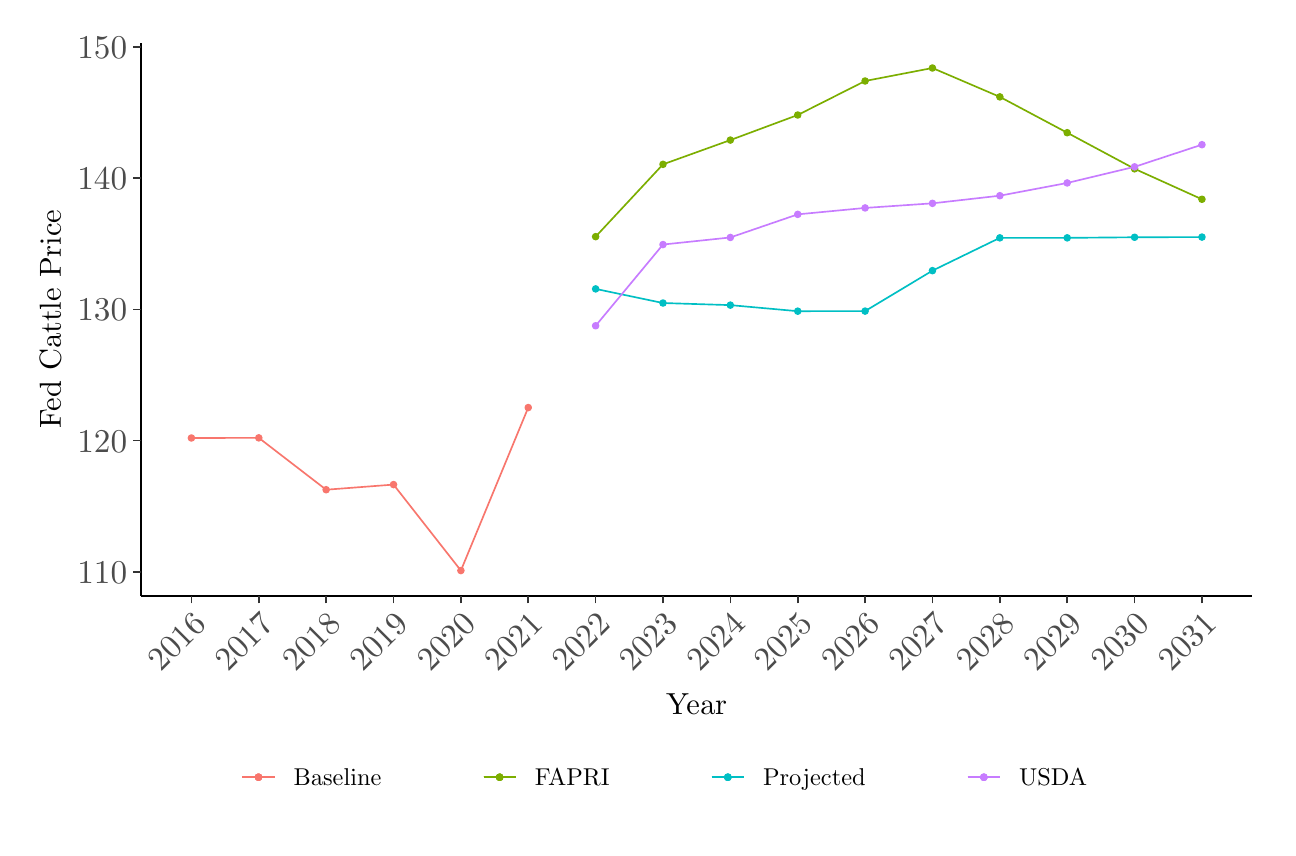
\begin{tikzpicture}[x=1pt,y=1pt]
\definecolor{fillColor}{RGB}{255,255,255}
\path[use as bounding box,fill=fillColor,fill opacity=0.00] (0,0) rectangle (448.07,289.08);
\begin{scope}
\path[clip] (  0.00,  0.00) rectangle (448.07,289.08);
\definecolor{drawColor}{RGB}{255,255,255}
\definecolor{fillColor}{RGB}{255,255,255}

\path[draw=drawColor,line width= 0.6pt,line join=round,line cap=round,fill=fillColor] (  0.00, -0.00) rectangle (448.07,289.08);
\end{scope}
\begin{scope}
\path[clip] ( 40.91, 83.83) rectangle (442.57,283.58);
\definecolor{fillColor}{RGB}{255,255,255}

\path[fill=fillColor] ( 40.91, 83.83) rectangle (442.57,283.58);
\definecolor{drawColor}{RGB}{248,118,109}

\path[draw=drawColor,line width= 0.6pt,line join=round] ( 59.17,140.81) --
	( 83.51,140.86) --
	(107.85,122.12) --
	(132.20,123.97) --
	(156.54, 92.91) --
	(180.88,151.81);
\definecolor{fillColor}{RGB}{248,118,109}

\path[draw=drawColor,line width= 0.4pt,line join=round,line cap=round,fill=fillColor] ( 59.17,140.81) circle (  1.16);

\path[draw=drawColor,line width= 0.4pt,line join=round,line cap=round,fill=fillColor] ( 83.51,140.86) circle (  1.16);

\path[draw=drawColor,line width= 0.4pt,line join=round,line cap=round,fill=fillColor] (107.85,122.12) circle (  1.16);

\path[draw=drawColor,line width= 0.4pt,line join=round,line cap=round,fill=fillColor] (132.20,123.97) circle (  1.16);

\path[draw=drawColor,line width= 0.4pt,line join=round,line cap=round,fill=fillColor] (156.54, 92.91) circle (  1.16);

\path[draw=drawColor,line width= 0.4pt,line join=round,line cap=round,fill=fillColor] (180.88,151.81) circle (  1.16);
\definecolor{drawColor}{RGB}{0,191,196}

\path[draw=drawColor,line width= 0.6pt,line join=round] (205.23,194.68) --
	(229.57,189.58) --
	(253.91,188.82) --
	(278.26,186.63) --
	(302.60,186.66) --
	(326.94,201.28) --
	(351.29,213.13) --
	(375.63,213.13) --
	(399.97,213.34) --
	(424.32,213.41);
\definecolor{fillColor}{RGB}{0,191,196}

\path[draw=drawColor,line width= 0.4pt,line join=round,line cap=round,fill=fillColor] (205.23,194.68) circle (  1.16);

\path[draw=drawColor,line width= 0.4pt,line join=round,line cap=round,fill=fillColor] (229.57,189.58) circle (  1.16);

\path[draw=drawColor,line width= 0.4pt,line join=round,line cap=round,fill=fillColor] (253.91,188.82) circle (  1.16);

\path[draw=drawColor,line width= 0.4pt,line join=round,line cap=round,fill=fillColor] (278.26,186.63) circle (  1.16);

\path[draw=drawColor,line width= 0.4pt,line join=round,line cap=round,fill=fillColor] (302.60,186.66) circle (  1.16);

\path[draw=drawColor,line width= 0.4pt,line join=round,line cap=round,fill=fillColor] (326.94,201.28) circle (  1.16);

\path[draw=drawColor,line width= 0.4pt,line join=round,line cap=round,fill=fillColor] (351.29,213.13) circle (  1.16);

\path[draw=drawColor,line width= 0.4pt,line join=round,line cap=round,fill=fillColor] (375.63,213.13) circle (  1.16);

\path[draw=drawColor,line width= 0.4pt,line join=round,line cap=round,fill=fillColor] (399.97,213.34) circle (  1.16);

\path[draw=drawColor,line width= 0.4pt,line join=round,line cap=round,fill=fillColor] (424.32,213.41) circle (  1.16);
\definecolor{drawColor}{RGB}{124,174,0}

\path[draw=drawColor,line width= 0.6pt,line join=round] (205.23,213.56) --
	(229.57,239.69) --
	(253.91,248.46) --
	(278.26,257.52) --
	(302.60,269.81) --
	(326.94,274.50) --
	(351.29,264.07) --
	(375.63,251.12) --
	(399.97,238.08) --
	(424.32,227.07);
\definecolor{fillColor}{RGB}{124,174,0}

\path[draw=drawColor,line width= 0.4pt,line join=round,line cap=round,fill=fillColor] (205.23,213.56) circle (  1.16);

\path[draw=drawColor,line width= 0.4pt,line join=round,line cap=round,fill=fillColor] (229.57,239.69) circle (  1.16);

\path[draw=drawColor,line width= 0.4pt,line join=round,line cap=round,fill=fillColor] (253.91,248.46) circle (  1.16);

\path[draw=drawColor,line width= 0.4pt,line join=round,line cap=round,fill=fillColor] (278.26,257.52) circle (  1.16);

\path[draw=drawColor,line width= 0.4pt,line join=round,line cap=round,fill=fillColor] (302.60,269.81) circle (  1.16);

\path[draw=drawColor,line width= 0.4pt,line join=round,line cap=round,fill=fillColor] (326.94,274.50) circle (  1.16);

\path[draw=drawColor,line width= 0.4pt,line join=round,line cap=round,fill=fillColor] (351.29,264.07) circle (  1.16);

\path[draw=drawColor,line width= 0.4pt,line join=round,line cap=round,fill=fillColor] (375.63,251.12) circle (  1.16);

\path[draw=drawColor,line width= 0.4pt,line join=round,line cap=round,fill=fillColor] (399.97,238.08) circle (  1.16);

\path[draw=drawColor,line width= 0.4pt,line join=round,line cap=round,fill=fillColor] (424.32,227.07) circle (  1.16);
\definecolor{drawColor}{RGB}{199,124,255}

\path[draw=drawColor,line width= 0.6pt,line join=round] (205.23,181.36) --
	(229.57,210.71) --
	(253.91,213.27) --
	(278.26,221.62) --
	(302.60,223.94) --
	(326.94,225.60) --
	(351.29,228.36) --
	(375.63,232.96) --
	(399.97,238.79) --
	(424.32,246.80);
\definecolor{fillColor}{RGB}{199,124,255}

\path[draw=drawColor,line width= 0.4pt,line join=round,line cap=round,fill=fillColor] (205.23,181.36) circle (  1.16);

\path[draw=drawColor,line width= 0.4pt,line join=round,line cap=round,fill=fillColor] (229.57,210.71) circle (  1.16);

\path[draw=drawColor,line width= 0.4pt,line join=round,line cap=round,fill=fillColor] (253.91,213.27) circle (  1.16);

\path[draw=drawColor,line width= 0.4pt,line join=round,line cap=round,fill=fillColor] (278.26,221.62) circle (  1.16);

\path[draw=drawColor,line width= 0.4pt,line join=round,line cap=round,fill=fillColor] (302.60,223.94) circle (  1.16);

\path[draw=drawColor,line width= 0.4pt,line join=round,line cap=round,fill=fillColor] (326.94,225.60) circle (  1.16);

\path[draw=drawColor,line width= 0.4pt,line join=round,line cap=round,fill=fillColor] (351.29,228.36) circle (  1.16);

\path[draw=drawColor,line width= 0.4pt,line join=round,line cap=round,fill=fillColor] (375.63,232.96) circle (  1.16);

\path[draw=drawColor,line width= 0.4pt,line join=round,line cap=round,fill=fillColor] (399.97,238.79) circle (  1.16);

\path[draw=drawColor,line width= 0.4pt,line join=round,line cap=round,fill=fillColor] (424.32,246.80) circle (  1.16);
\end{scope}
\begin{scope}
\path[clip] (  0.00,  0.00) rectangle (448.07,289.08);
\definecolor{drawColor}{RGB}{0,0,0}

\path[draw=drawColor,line width= 0.6pt,line join=round] ( 40.91, 83.83) --
	( 40.91,283.58);
\end{scope}
\begin{scope}
\path[clip] (  0.00,  0.00) rectangle (448.07,289.08);
\definecolor{drawColor}{gray}{0.30}

\node[text=drawColor,anchor=base east,inner sep=0pt, outer sep=0pt, scale=  1.20] at ( 35.96, 88.30) {110};

\node[text=drawColor,anchor=base east,inner sep=0pt, outer sep=0pt, scale=  1.20] at ( 35.96,135.73) {120};

\node[text=drawColor,anchor=base east,inner sep=0pt, outer sep=0pt, scale=  1.20] at ( 35.96,183.15) {130};

\node[text=drawColor,anchor=base east,inner sep=0pt, outer sep=0pt, scale=  1.20] at ( 35.96,230.58) {140};

\node[text=drawColor,anchor=base east,inner sep=0pt, outer sep=0pt, scale=  1.20] at ( 35.96,278.00) {150};
\end{scope}
\begin{scope}
\path[clip] (  0.00,  0.00) rectangle (448.07,289.08);
\definecolor{drawColor}{gray}{0.20}

\path[draw=drawColor,line width= 0.6pt,line join=round] ( 38.16, 92.43) --
	( 40.91, 92.43);

\path[draw=drawColor,line width= 0.6pt,line join=round] ( 38.16,139.86) --
	( 40.91,139.86);

\path[draw=drawColor,line width= 0.6pt,line join=round] ( 38.16,187.28) --
	( 40.91,187.28);

\path[draw=drawColor,line width= 0.6pt,line join=round] ( 38.16,234.71) --
	( 40.91,234.71);

\path[draw=drawColor,line width= 0.6pt,line join=round] ( 38.16,282.14) --
	( 40.91,282.14);
\end{scope}
\begin{scope}
\path[clip] (  0.00,  0.00) rectangle (448.07,289.08);
\definecolor{drawColor}{RGB}{0,0,0}

\path[draw=drawColor,line width= 0.6pt,line join=round] ( 40.91, 83.83) --
	(442.57, 83.83);
\end{scope}
\begin{scope}
\path[clip] (  0.00,  0.00) rectangle (448.07,289.08);
\definecolor{drawColor}{gray}{0.20}

\path[draw=drawColor,line width= 0.6pt,line join=round] ( 59.17, 81.08) --
	( 59.17, 83.83);

\path[draw=drawColor,line width= 0.6pt,line join=round] ( 83.51, 81.08) --
	( 83.51, 83.83);

\path[draw=drawColor,line width= 0.6pt,line join=round] (107.85, 81.08) --
	(107.85, 83.83);

\path[draw=drawColor,line width= 0.6pt,line join=round] (132.20, 81.08) --
	(132.20, 83.83);

\path[draw=drawColor,line width= 0.6pt,line join=round] (156.54, 81.08) --
	(156.54, 83.83);

\path[draw=drawColor,line width= 0.6pt,line join=round] (180.88, 81.08) --
	(180.88, 83.83);

\path[draw=drawColor,line width= 0.6pt,line join=round] (205.23, 81.08) --
	(205.23, 83.83);

\path[draw=drawColor,line width= 0.6pt,line join=round] (229.57, 81.08) --
	(229.57, 83.83);

\path[draw=drawColor,line width= 0.6pt,line join=round] (253.91, 81.08) --
	(253.91, 83.83);

\path[draw=drawColor,line width= 0.6pt,line join=round] (278.26, 81.08) --
	(278.26, 83.83);

\path[draw=drawColor,line width= 0.6pt,line join=round] (302.60, 81.08) --
	(302.60, 83.83);

\path[draw=drawColor,line width= 0.6pt,line join=round] (326.94, 81.08) --
	(326.94, 83.83);

\path[draw=drawColor,line width= 0.6pt,line join=round] (351.29, 81.08) --
	(351.29, 83.83);

\path[draw=drawColor,line width= 0.6pt,line join=round] (375.63, 81.08) --
	(375.63, 83.83);

\path[draw=drawColor,line width= 0.6pt,line join=round] (399.97, 81.08) --
	(399.97, 83.83);

\path[draw=drawColor,line width= 0.6pt,line join=round] (424.32, 81.08) --
	(424.32, 83.83);
\end{scope}
\begin{scope}
\path[clip] (  0.00,  0.00) rectangle (448.07,289.08);
\definecolor{drawColor}{gray}{0.30}

\node[text=drawColor,rotate= 45.00,anchor=base east,inner sep=0pt, outer sep=0pt, scale=  1.20] at ( 65.01, 73.03) {2016};

\node[text=drawColor,rotate= 45.00,anchor=base east,inner sep=0pt, outer sep=0pt, scale=  1.20] at ( 89.35, 73.03) {2017};

\node[text=drawColor,rotate= 45.00,anchor=base east,inner sep=0pt, outer sep=0pt, scale=  1.20] at (113.70, 73.03) {2018};

\node[text=drawColor,rotate= 45.00,anchor=base east,inner sep=0pt, outer sep=0pt, scale=  1.20] at (138.04, 73.03) {2019};

\node[text=drawColor,rotate= 45.00,anchor=base east,inner sep=0pt, outer sep=0pt, scale=  1.20] at (162.38, 73.03) {2020};

\node[text=drawColor,rotate= 45.00,anchor=base east,inner sep=0pt, outer sep=0pt, scale=  1.20] at (186.73, 73.03) {2021};

\node[text=drawColor,rotate= 45.00,anchor=base east,inner sep=0pt, outer sep=0pt, scale=  1.20] at (211.07, 73.03) {2022};

\node[text=drawColor,rotate= 45.00,anchor=base east,inner sep=0pt, outer sep=0pt, scale=  1.20] at (235.41, 73.03) {2023};

\node[text=drawColor,rotate= 45.00,anchor=base east,inner sep=0pt, outer sep=0pt, scale=  1.20] at (259.76, 73.03) {2024};

\node[text=drawColor,rotate= 45.00,anchor=base east,inner sep=0pt, outer sep=0pt, scale=  1.20] at (284.10, 73.03) {2025};

\node[text=drawColor,rotate= 45.00,anchor=base east,inner sep=0pt, outer sep=0pt, scale=  1.20] at (308.44, 73.03) {2026};

\node[text=drawColor,rotate= 45.00,anchor=base east,inner sep=0pt, outer sep=0pt, scale=  1.20] at (332.79, 73.03) {2027};

\node[text=drawColor,rotate= 45.00,anchor=base east,inner sep=0pt, outer sep=0pt, scale=  1.20] at (357.13, 73.03) {2028};

\node[text=drawColor,rotate= 45.00,anchor=base east,inner sep=0pt, outer sep=0pt, scale=  1.20] at (381.47, 73.03) {2029};

\node[text=drawColor,rotate= 45.00,anchor=base east,inner sep=0pt, outer sep=0pt, scale=  1.20] at (405.82, 73.03) {2030};

\node[text=drawColor,rotate= 45.00,anchor=base east,inner sep=0pt, outer sep=0pt, scale=  1.20] at (430.16, 73.03) {2031};
\end{scope}
\begin{scope}
\path[clip] (  0.00,  0.00) rectangle (448.07,289.08);
\definecolor{drawColor}{RGB}{0,0,0}

\node[text=drawColor,anchor=base,inner sep=0pt, outer sep=0pt, scale=  1.10] at (241.74, 40.88) {Year};
\end{scope}
\begin{scope}
\path[clip] (  0.00,  0.00) rectangle (448.07,289.08);
\definecolor{drawColor}{RGB}{0,0,0}

\node[text=drawColor,rotate= 90.00,anchor=base,inner sep=0pt, outer sep=0pt, scale=  1.10] at ( 12.01,183.70) {Fed Cattle Price};
\end{scope}
\begin{scope}
\path[clip] (  0.00,  0.00) rectangle (448.07,289.08);
\definecolor{fillColor}{RGB}{255,255,255}

\path[fill=fillColor] ( 65.18,  5.50) rectangle (418.31, 30.95);
\end{scope}
\begin{scope}
\path[clip] (  0.00,  0.00) rectangle (448.07,289.08);
\definecolor{drawColor}{RGB}{248,118,109}

\path[draw=drawColor,line width= 0.6pt,line join=round] ( 77.62, 18.23) -- ( 89.19, 18.23);
\end{scope}
\begin{scope}
\path[clip] (  0.00,  0.00) rectangle (448.07,289.08);
\definecolor{drawColor}{RGB}{248,118,109}
\definecolor{fillColor}{RGB}{248,118,109}

\path[draw=drawColor,line width= 0.4pt,line join=round,line cap=round,fill=fillColor] ( 83.41, 18.23) circle (  1.16);
\end{scope}
\begin{scope}
\path[clip] (  0.00,  0.00) rectangle (448.07,289.08);
\definecolor{drawColor}{RGB}{248,118,109}

\path[draw=drawColor,line width= 0.6pt,line join=round] ( 77.62, 18.23) -- ( 89.19, 18.23);
\end{scope}
\begin{scope}
\path[clip] (  0.00,  0.00) rectangle (448.07,289.08);
\definecolor{drawColor}{RGB}{248,118,109}
\definecolor{fillColor}{RGB}{248,118,109}

\path[draw=drawColor,line width= 0.4pt,line join=round,line cap=round,fill=fillColor] ( 83.41, 18.23) circle (  1.16);
\end{scope}
\begin{scope}
\path[clip] (  0.00,  0.00) rectangle (448.07,289.08);
\definecolor{drawColor}{RGB}{248,118,109}

\path[draw=drawColor,line width= 0.6pt,line join=round] ( 77.62, 18.23) -- ( 89.19, 18.23);
\end{scope}
\begin{scope}
\path[clip] (  0.00,  0.00) rectangle (448.07,289.08);
\definecolor{drawColor}{RGB}{248,118,109}
\definecolor{fillColor}{RGB}{248,118,109}

\path[draw=drawColor,line width= 0.4pt,line join=round,line cap=round,fill=fillColor] ( 83.41, 18.23) circle (  1.16);
\end{scope}
\begin{scope}
\path[clip] (  0.00,  0.00) rectangle (448.07,289.08);
\definecolor{drawColor}{RGB}{248,118,109}

\path[draw=drawColor,line width= 0.6pt,line join=round] ( 77.62, 18.23) -- ( 89.19, 18.23);
\end{scope}
\begin{scope}
\path[clip] (  0.00,  0.00) rectangle (448.07,289.08);
\definecolor{drawColor}{RGB}{248,118,109}
\definecolor{fillColor}{RGB}{248,118,109}

\path[draw=drawColor,line width= 0.4pt,line join=round,line cap=round,fill=fillColor] ( 83.41, 18.23) circle (  1.16);
\end{scope}
\begin{scope}
\path[clip] (  0.00,  0.00) rectangle (448.07,289.08);
\definecolor{drawColor}{RGB}{124,174,0}

\path[draw=drawColor,line width= 0.6pt,line join=round] (164.77, 18.23) -- (176.34, 18.23);
\end{scope}
\begin{scope}
\path[clip] (  0.00,  0.00) rectangle (448.07,289.08);
\definecolor{drawColor}{RGB}{124,174,0}
\definecolor{fillColor}{RGB}{124,174,0}

\path[draw=drawColor,line width= 0.4pt,line join=round,line cap=round,fill=fillColor] (170.56, 18.23) circle (  1.16);
\end{scope}
\begin{scope}
\path[clip] (  0.00,  0.00) rectangle (448.07,289.08);
\definecolor{drawColor}{RGB}{124,174,0}

\path[draw=drawColor,line width= 0.6pt,line join=round] (164.77, 18.23) -- (176.34, 18.23);
\end{scope}
\begin{scope}
\path[clip] (  0.00,  0.00) rectangle (448.07,289.08);
\definecolor{drawColor}{RGB}{124,174,0}
\definecolor{fillColor}{RGB}{124,174,0}

\path[draw=drawColor,line width= 0.4pt,line join=round,line cap=round,fill=fillColor] (170.56, 18.23) circle (  1.16);
\end{scope}
\begin{scope}
\path[clip] (  0.00,  0.00) rectangle (448.07,289.08);
\definecolor{drawColor}{RGB}{124,174,0}

\path[draw=drawColor,line width= 0.6pt,line join=round] (164.77, 18.23) -- (176.34, 18.23);
\end{scope}
\begin{scope}
\path[clip] (  0.00,  0.00) rectangle (448.07,289.08);
\definecolor{drawColor}{RGB}{124,174,0}
\definecolor{fillColor}{RGB}{124,174,0}

\path[draw=drawColor,line width= 0.4pt,line join=round,line cap=round,fill=fillColor] (170.56, 18.23) circle (  1.16);
\end{scope}
\begin{scope}
\path[clip] (  0.00,  0.00) rectangle (448.07,289.08);
\definecolor{drawColor}{RGB}{124,174,0}

\path[draw=drawColor,line width= 0.6pt,line join=round] (164.77, 18.23) -- (176.34, 18.23);
\end{scope}
\begin{scope}
\path[clip] (  0.00,  0.00) rectangle (448.07,289.08);
\definecolor{drawColor}{RGB}{124,174,0}
\definecolor{fillColor}{RGB}{124,174,0}

\path[draw=drawColor,line width= 0.4pt,line join=round,line cap=round,fill=fillColor] (170.56, 18.23) circle (  1.16);
\end{scope}
\begin{scope}
\path[clip] (  0.00,  0.00) rectangle (448.07,289.08);
\definecolor{drawColor}{RGB}{0,191,196}

\path[draw=drawColor,line width= 0.6pt,line join=round] (247.23, 18.23) -- (258.80, 18.23);
\end{scope}
\begin{scope}
\path[clip] (  0.00,  0.00) rectangle (448.07,289.08);
\definecolor{drawColor}{RGB}{0,191,196}
\definecolor{fillColor}{RGB}{0,191,196}

\path[draw=drawColor,line width= 0.4pt,line join=round,line cap=round,fill=fillColor] (253.01, 18.23) circle (  1.16);
\end{scope}
\begin{scope}
\path[clip] (  0.00,  0.00) rectangle (448.07,289.08);
\definecolor{drawColor}{RGB}{0,191,196}

\path[draw=drawColor,line width= 0.6pt,line join=round] (247.23, 18.23) -- (258.80, 18.23);
\end{scope}
\begin{scope}
\path[clip] (  0.00,  0.00) rectangle (448.07,289.08);
\definecolor{drawColor}{RGB}{0,191,196}
\definecolor{fillColor}{RGB}{0,191,196}

\path[draw=drawColor,line width= 0.4pt,line join=round,line cap=round,fill=fillColor] (253.01, 18.23) circle (  1.16);
\end{scope}
\begin{scope}
\path[clip] (  0.00,  0.00) rectangle (448.07,289.08);
\definecolor{drawColor}{RGB}{0,191,196}

\path[draw=drawColor,line width= 0.6pt,line join=round] (247.23, 18.23) -- (258.80, 18.23);
\end{scope}
\begin{scope}
\path[clip] (  0.00,  0.00) rectangle (448.07,289.08);
\definecolor{drawColor}{RGB}{0,191,196}
\definecolor{fillColor}{RGB}{0,191,196}

\path[draw=drawColor,line width= 0.4pt,line join=round,line cap=round,fill=fillColor] (253.01, 18.23) circle (  1.16);
\end{scope}
\begin{scope}
\path[clip] (  0.00,  0.00) rectangle (448.07,289.08);
\definecolor{drawColor}{RGB}{0,191,196}

\path[draw=drawColor,line width= 0.6pt,line join=round] (247.23, 18.23) -- (258.80, 18.23);
\end{scope}
\begin{scope}
\path[clip] (  0.00,  0.00) rectangle (448.07,289.08);
\definecolor{drawColor}{RGB}{0,191,196}
\definecolor{fillColor}{RGB}{0,191,196}

\path[draw=drawColor,line width= 0.4pt,line join=round,line cap=round,fill=fillColor] (253.01, 18.23) circle (  1.16);
\end{scope}
\begin{scope}
\path[clip] (  0.00,  0.00) rectangle (448.07,289.08);
\definecolor{drawColor}{RGB}{199,124,255}

\path[draw=drawColor,line width= 0.6pt,line join=round] (339.74, 18.23) -- (351.30, 18.23);
\end{scope}
\begin{scope}
\path[clip] (  0.00,  0.00) rectangle (448.07,289.08);
\definecolor{drawColor}{RGB}{199,124,255}
\definecolor{fillColor}{RGB}{199,124,255}

\path[draw=drawColor,line width= 0.4pt,line join=round,line cap=round,fill=fillColor] (345.52, 18.23) circle (  1.16);
\end{scope}
\begin{scope}
\path[clip] (  0.00,  0.00) rectangle (448.07,289.08);
\definecolor{drawColor}{RGB}{199,124,255}

\path[draw=drawColor,line width= 0.6pt,line join=round] (339.74, 18.23) -- (351.30, 18.23);
\end{scope}
\begin{scope}
\path[clip] (  0.00,  0.00) rectangle (448.07,289.08);
\definecolor{drawColor}{RGB}{199,124,255}
\definecolor{fillColor}{RGB}{199,124,255}

\path[draw=drawColor,line width= 0.4pt,line join=round,line cap=round,fill=fillColor] (345.52, 18.23) circle (  1.16);
\end{scope}
\begin{scope}
\path[clip] (  0.00,  0.00) rectangle (448.07,289.08);
\definecolor{drawColor}{RGB}{199,124,255}

\path[draw=drawColor,line width= 0.6pt,line join=round] (339.74, 18.23) -- (351.30, 18.23);
\end{scope}
\begin{scope}
\path[clip] (  0.00,  0.00) rectangle (448.07,289.08);
\definecolor{drawColor}{RGB}{199,124,255}
\definecolor{fillColor}{RGB}{199,124,255}

\path[draw=drawColor,line width= 0.4pt,line join=round,line cap=round,fill=fillColor] (345.52, 18.23) circle (  1.16);
\end{scope}
\begin{scope}
\path[clip] (  0.00,  0.00) rectangle (448.07,289.08);
\definecolor{drawColor}{RGB}{199,124,255}

\path[draw=drawColor,line width= 0.6pt,line join=round] (339.74, 18.23) -- (351.30, 18.23);
\end{scope}
\begin{scope}
\path[clip] (  0.00,  0.00) rectangle (448.07,289.08);
\definecolor{drawColor}{RGB}{199,124,255}
\definecolor{fillColor}{RGB}{199,124,255}

\path[draw=drawColor,line width= 0.4pt,line join=round,line cap=round,fill=fillColor] (345.52, 18.23) circle (  1.16);
\end{scope}
\begin{scope}
\path[clip] (  0.00,  0.00) rectangle (448.07,289.08);
\definecolor{drawColor}{RGB}{0,0,0}

\node[text=drawColor,anchor=base west,inner sep=0pt, outer sep=0pt, scale=  0.88] at ( 96.13, 15.20) {Baseline};
\end{scope}
\begin{scope}
\path[clip] (  0.00,  0.00) rectangle (448.07,289.08);
\definecolor{drawColor}{RGB}{0,0,0}

\node[text=drawColor,anchor=base west,inner sep=0pt, outer sep=0pt, scale=  0.88] at (183.28, 15.20) {FAPRI};
\end{scope}
\begin{scope}
\path[clip] (  0.00,  0.00) rectangle (448.07,289.08);
\definecolor{drawColor}{RGB}{0,0,0}

\node[text=drawColor,anchor=base west,inner sep=0pt, outer sep=0pt, scale=  0.88] at (265.74, 15.20) {Projected};
\end{scope}
\begin{scope}
\path[clip] (  0.00,  0.00) rectangle (448.07,289.08);
\definecolor{drawColor}{RGB}{0,0,0}

\node[text=drawColor,anchor=base west,inner sep=0pt, outer sep=0pt, scale=  0.88] at (358.24, 15.20) {USDA};
\end{scope}
\end{tikzpicture}
